%% 
%% Master Thesis
%% Autor: Martin Wichmann
%% 
%% Todo:
%% - Danksagung
%% - Cite auf mein GitHub ändern oder so?!
%% - Portabilität PC VM auf embedded Hypervisor
%% - Relevanz für Testen und Entwicklungsprozess
%% - Autosar oder AUTOSAR?!


\documentclass[
  a4paper,					    % a4paper (sic!)
  %BCOR10mm,				    % Korrektur des innneren Randes bei Bindung (Bindungskorrektur)
  %DIV12,					    % je groesser die Zahl, desto kleiner der Rand
  %11pt,        			    % Schriftgroesse
  %oneside,
  twoside,
  %openright,   				% doppelseitig und jedes Kapitel faengt auf der rechten Seite an
  %pagesize,					% schreibt die Seitengroesseninformationen in die PDF Datei
  DIV=calc,     				% KOMA-Script soll den optimalen Satzspiegel berechnen
  %DIVclassic, 					% mittelalterlicher Buchseitenkanon
  %headsepline,					% Trennlinie
  %footsepline,					% Trennlinie
  %headtopline,					% Trennlinie
  %footbotline,					% Trennlinie
  %noonelinecaption,			% setzt die Bildueberschrift unabhaengig von der Laenge immer linksbuendig
  %liststotoc,
  %idxtotoc,
  bibliography=totoc,
  %bibtotocnumbered, liststotocnumbered,
  %liststotoc, idxtotoc, bibtotoc,
  %tablecaptionbelow,
  %tablecaptionabove,	        % Tabellenbeschriftung unter oder oben
  %abstracton,  				% Überschrift der Zusammenfassung aktivieren
  %chapterprefix,				% "Kapitel xx" vor jeder Kapitelueberschrift
  %cleardoublestandard,
  %cleardoubleplain,
  cleardoublepage=empty,
  %smallheadings,
  %normalheadings,
  %makeidx,
  ngerman,     					% allen Paketen die Hauptsprache mitteilen
  %draft       					% draft version  
  final       					% final version
]{scrbook}	
%%%%%%%%%%%%%%% Grundlegendes %%%%%%%%%%%%%%%
\usepackage[utf8]{inputenc}
\usepackage[T1]{fontenc}
\usepackage[english,ngerman]{babel} 	% Unterstuezung fuer englisch und deutsch
\usepackage{setspace}			% erlaubt 1 1/2 fachen Zeilenabstand
%%%%%%%%%%%%%%% Tabellen %%%%%%%%%%%%%%%
%\usepackage{array}
%\usepackage{tabularx}
\usepackage{booktabs}			% \toprule, \midrule und \bottomrule in Tabellen
\usepackage{multirow}
%%%%%%%%%%%%%%% Mathe %%%%%%%%%%%%%%%
%\usepackage{amsmath, amsthm, amscd, amssymb, amsfonts}
%\usepackage{ziffer}
%\usepackage{icomma}
%%%%%%%%%%%%%%% Typografie %%%%%%%%%%%%%%%
%\usepackage{mparhack}			% workaround for a LaTeX bug in marginpars
\usepackage{ellipsis}			% fix uneven spacing around ellipses in LaTeX text mode.
\usepackage{microtype} 			% optischer Randausgleich (font expansion and character protrusion)
%%%%%%%%%%%%%%% Schriften %%%%%%%%%%%%%%%
\usepackage{lmodern}
%\usepackage{textcomp} 			% Sonderzeichen
%\usepackage{mathcomp}
%\usepackage{chemsym}
%%%%%%%%%%%%%%% Sonstiges %%%%%%%%%%%%%%%
%\usepackage{url}
\usepackage{scrhack}            % KOMA Paket um zussammenarbeit mit anderen Paket (listings) zu verbessern
\usepackage{listings}			% Code-Abschnitt mit Syntax-Highlighting
\lstset{
%language=C,
breaklines=true,
breakatwhitespace=true
basicstyle=\footnotesize,
numbers=left,
numberstyle=\footnotesize,
stepnumber=2,
numbersep=5pt,
extendedchars=true,
inputencoding=utf8,
breakindent=30pt,
escapeinside={\%(}{\%)},
%xleftmargin=20pt				% Einrückung der listings
}
%\usepackage{color} 			% Farben
%%%%%%%%%%%%%%% Grafiken %%%%%%%%%%%%%%%
\usepackage[pdftex]{graphicx}	% das pdftex soll das Handling von Bildern verbessern
\graphicspath{{images/}}		% Bilder im Verzeichnis images suchen
\usepackage{wrapfig}
%\usepackage[hang]{subfigure}	% Subabbildungen
%\usepackage{tikz}				% zum Zeichnen (Frontend zu PGF)
\usepackage{pgfgantt}           % pgf verwenden um Gantt Diagramme zu erstellen
%\usepackage{rotating} 			% fuer gedrehte Tabellen und Bilder
%\usepackage{pdfpages}
\usepackage[
  pdftex,
  bookmarks, bookmarksopen, bookmarksopenlevel=1, bookmarksnumbered=true,
  pdfpagemode={UseNone},		% UseNone, FullScreen, UseThumbs, UseOutlines, (UseOC, UseAttachments)
  pdfpagelayout={TwoPageRight},	% SinglePage, OneColumn, TwoColumnLeft, TwoColumnRight, TwoPageLeft, TwoPageRight
  plainpages=false, 
  pdfkeywords={},
  pdfsubject={},
  pdftitle={Master-Arbeit},
  pdfauthor={Martin Wichmann}
]{hyperref}
%%%%%%%%%%%%%%% Zitieren und Index %%%%%%%%%%%%%%%
% Ich habe im Internet gelesen, dass cite nach hyperref stehen soll?!
\usepackage[numbers]{natbib}
% Index:
%\usepackage{makeidx}					% Paket für die Indexerstellung
%\makeindex
% Glossar:
%\usepackage[style=super, header=none, border=none, number=none, cols=2, toc=true]{glossary}
%\usepackage[style=altlist, number=none]{glossary}
%\makeglossary
% Benutzung des Glossars: \glossary{name={Schnauze}, description={Fachausdruck für die Hundenase.},}
%                         \glossary{name={Knochen}, description={Lieblingsspeise eines jeden Hundes.},}
%%%%%%%%%%%%%%%%%%%%%%%%%%%%%%%%%%%%%%%%%%%%%%%%%%%%

%%%%%%%%%%%%%%%%%%%%%%%% Eigene Definitionen %%%%%%%%%%%%%%%%%%%%%%%%%%%%%%

%%% Bei Verwendung von BibTex: %%%%%%%%%%%%%%%%%%%%
\addto{\captionsngerman}{\renewcommand*{\bibname}{Quellenverzeichnis}}
% sonst
%\renewcommand{\bibname}{Quellenverzeichnis}

%%% Trennungen %%%%%%%%%%%%%%%%%%%%%%%%%%%%%%%%%%%%%%%%%%%
\hyphenation{}

%%% 1 1/2 fachen Zeilenabstand wählen %%%%%%%%%%%%%%%%%%%%
\onehalfspacing
\typearea[current]{calc}				% Neuberechnung des Satzspiegels

%%%%%%%%%%%%%%%%%%%%%%%%%%%% Begin document %%%%%%%%%%%%%%%%%%%%%%%%%%%%%%%
\begin{document}
\selectlanguage{ngerman}
\frontmatter

%%%%%%%%%%%%%%%%%%%%%%%%%%%%%%%%% Titel %%%%%%%%%%%%%%%%%%%%%%%%%%%%%%%%%%
\titlehead{\center{\large \textsc{Ostfalia Hochschule für angewandte Wissenschaften}}}
\subject{Master-Arbeit}
\title{Virtualisierung von Autosar Softwarekomponenten für die Erprobung}
\author{Martin Wichmann\\Matrikel 701\,277\,37}
\date{Eingereicht am TODO}
\publishers{Prüfer: 

  Prof. Dr.-Ing. Gert Bikker

  Prof. Dr.-Ing. Jürgen Kreyßig

  }

%\uppertitleback{%
%  Beteiligte Institutionen:\\
%  \parbox{0.5\textwidth}{%
%  \centering \includegraphics[width=3.5cm]{logofh} \\
%  Fakultät Informatik \\ Ostfalia Hochschule für angewandte Wissenschaften } \hfill
%}


% TODO: github cite in footnote ändern?!
\lowertitleback{Diese Arbeit wurde mit Hilfe von Freier Software erstellt: \\
Gesetzt mit Hilfe von {\KOMAScript} und {\LaTeX}. LibreOffice für die \\ Textverarbeitung und gedit als Editor. Xubuntu als offenes Betriebssystem. \\ \\ Diese Arbeit ist freigegeben unter der Creative Commons CC-BY-SA Lizenz\cite{CCBYSA} und ist im Internet erreichbar\cite{github}.
}
% TODO: evtl. qoute ändern ;-)
\dedication{Do or do not...there is no try!\\ \vspace{1cm}
\textit{Yoda}
}

\begin{singlespace}
\maketitle

%%%%%%%%%%%%%%%% Abstract %%%%%%%%%%%%%%%%%%%%%%%


\section*{Zusammenfassung}
\pdfbookmark[1]{Zusammenfassung}{Zussammenfassung}
TODO
\vfill

\foreignlanguage{english}{
\section*{Abstract}
TODO
\vfill
}


\thispagestyle{empty}

%%%%%%%%%%%%%%%%%%%%%%%%%%%%%% Verzeichnisse %%%%%%%%%%%%%%%%%%%%%%%%%%%%%%

\tableofcontents               	% Inhaltsverzeichnis
%\listoffigures               		% Abbildungsverzeichnis
%\listoftables             			% Tabellenverzeichnis
%\lstlistoflistings          		% Listenverzeichnis
%\listoflistings					% Quellcodeverzeichis
%\printglossary               		% Formelverzeichnis
\end{singlespace}


%%%%%%%%%%%%%%%%%%%%%%%%%%%%%% Zeilenabstand %%%%%%%%%%%%%%%%%%%%%%%%%%%%%%
% Das Setzen eines anderen Abstandes mitten im Dokument kann zu Fehlern führen (vgl. scrguide S. 30)
%\doublespacing
%\onehalfspacing
%\typearea[current]{last}					% stammt aus scrguide S. 30
%\typearea[current]{calc}					% Neuberechnung des Satzspiegels









%%%%%%%%%%%%%%%%%%%%%%%%%%%%%%% Einleitung %%%%%%%%%%%%%%%%%%%%%%%%%%%%%%%%%%
\mainmatter
\chapter{Einleitung}
\label{sec:Einleitung}
% TODO

Diese Master-Arbeit betrachtet die Möglichkeiten der Virtualisierung im Embedded Bereich anhand eines Fallbeispiels. Dieses Fallbeispiel wird im nächsten Kapitel vorgestellt. Anschließend werden die theoretischen Grundlagen erläutert und diskutiert. Die praktische Umsetzung des Fallbeispiels wird danach erläutert. Zum Schluss werden einige Aspekte werden einige Aspekte dieser Arbeit analysiert und die Relevanz für die Wirtschaft betrachtet.





%%%%%%%%%%%%%%%%%%%%%%%%%%%%%%% Vorstellung Fallbeispiel %%%%%%%%%%%%%%%%%%%%%%%%%%%%%%%%%%
% Gesamtes Modell darstellen
\chapter{Motivation und Planung}
\label{sec:MotivationPlanung}
% Motivation für Autosar und Virtualisierung
% Wodurch werden Systeme komplexer [SE_Autosar, Seite 11]
% Ein System partitionieren [SE_Autosar, Seite 27]

% Beispiel in dieser Arbeit
Das in dieser Master-Arbeit betrachtete Praxis-Beispiel ist eine Scheinwerfer-Steuerung inklusive User-Interface. Dies ist bewusst als minimal Beispiel konzipiert um den Fokus auf die Virtualisierung zu legen.

\begin{figure}[ht]
\centering
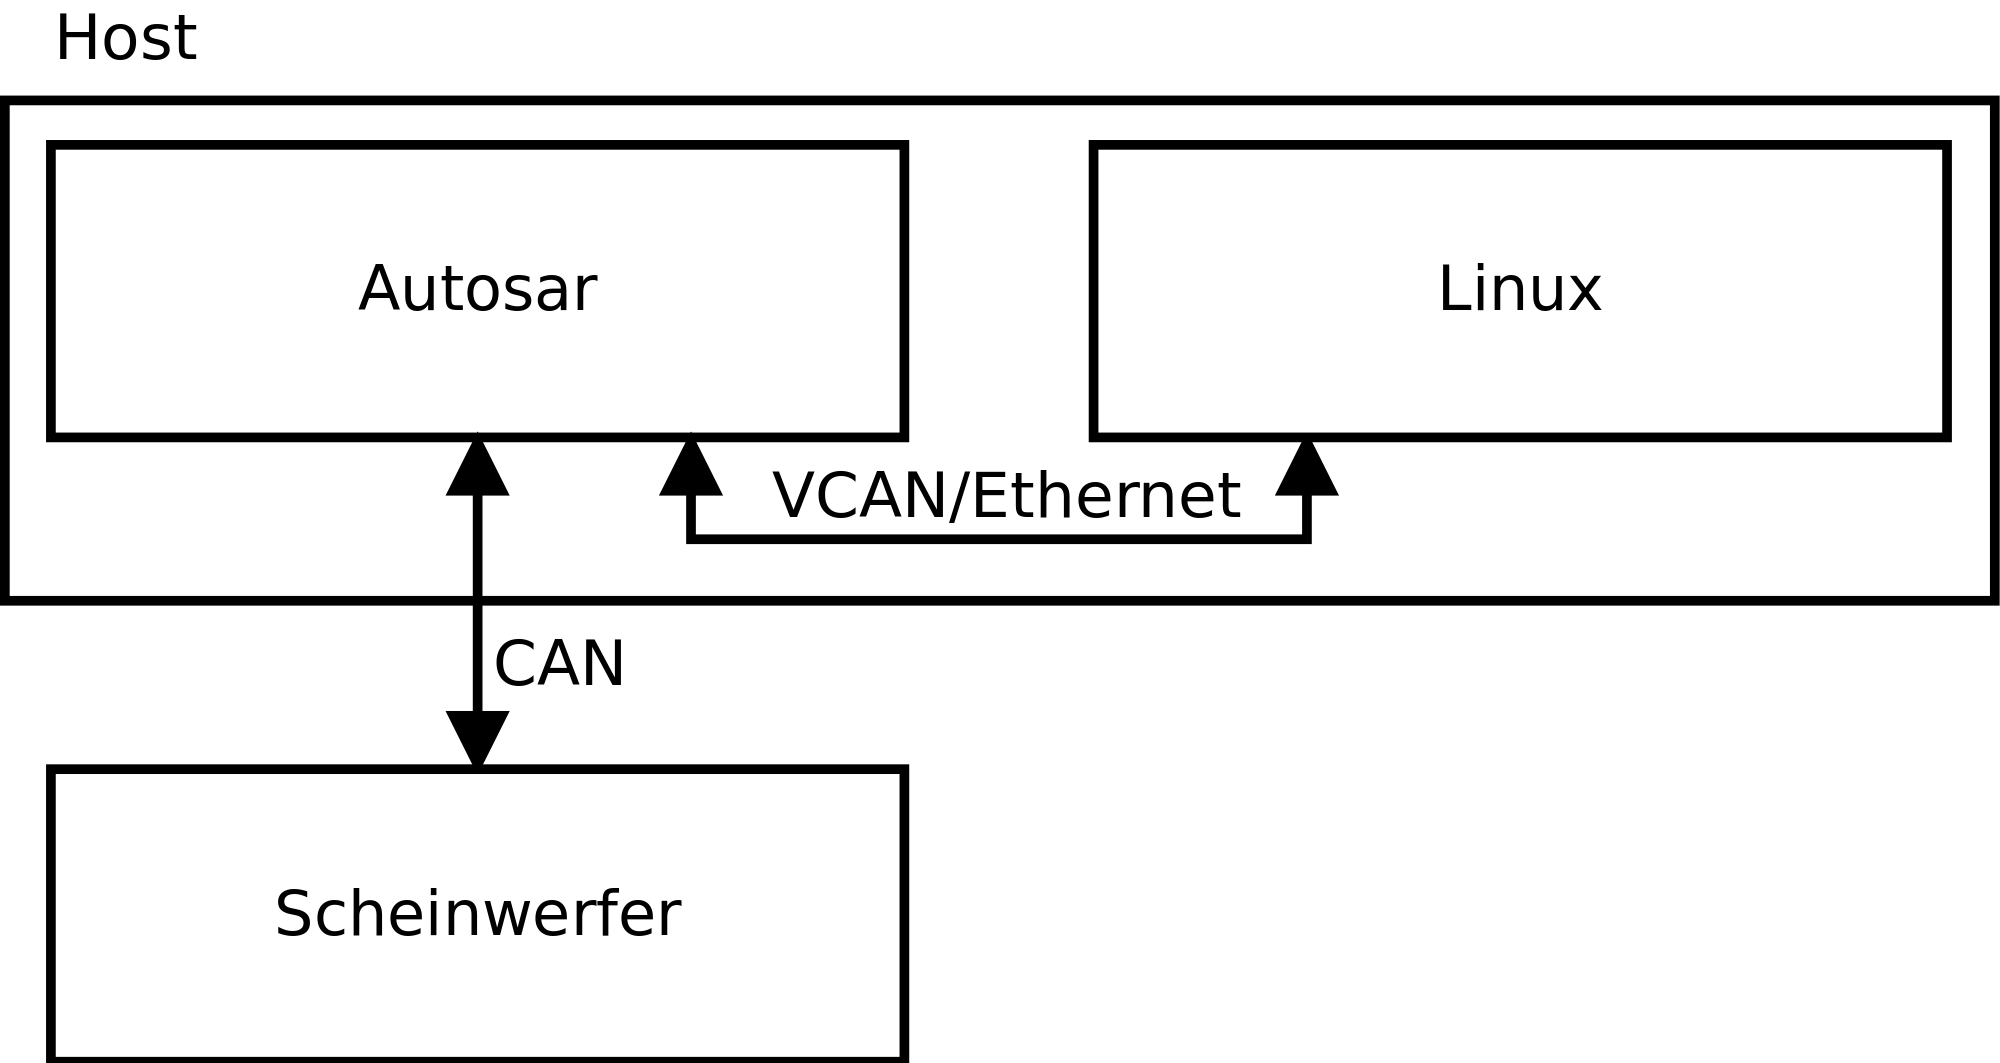
\includegraphics[width=0.8\textwidth]{overview.png}
\caption{Architektur}
\label{fig:arch}
\end{figure}

Die geplante Architektur der Scheinwerfer-Steuerung ist in Abbildung \ref{fig:arch} zu sehen. Dabei sind zwei getrennte Hardware Elemente zu sehen. Zum einen das Scheinwerfer-Steuergerät und zum anderen das in dieser Arbeit betrachtete System. Das Steuergerät übernimmt die direkte Steuerung der Scheinwerfer und ist per CAN-Bus mit dem anderen System verbunden.  Dieses beherbergt ein virtuelles Autosar und Linux auf einem Windows Host.

Aus dieser Architektur-Beschreibung lassen sich vier Kern-Bereiche dieser Master-Arbeit ableiten:

\begin{itemize}
    \item Virtualisierung von Autosar und Linux
    \item Kommunikation zwischen Linux und Autosar
    \item Kommunikation zwischen Autosar und Scheinwerfer
    \item Zugriff auf Hardware inklusive Betrachtung von Netzwerkmanagement
\end{itemize}

Hierbei ist zu beachten, dass das aktivieren des Netzwerkmanagements erst möglich ist, sobald eine Kommunikation zwischen Autosar und der Hardware möglich ist.

% TODO: Projektplanung
Da der Zeitaufwand für die einzelnen Phasen nur sehr schwer einzuschätzen ist, wird für jede Phase des Projektes ein Monat Arbeit vorgesehen. Dazu kommen noch ein Monat Evaluation und Sicherheitsbetrachtung des Systems und zum Schluss ein Monat Fertigstellen der schriftlichen Arbeit. Die Zeitplanung ist in einem Gantt-Diagramm in Abbildung \ref{fig:gantt} zu sehen. Jede Phase enthält die Vorbereitung, Umsetzung und Dokmentation des entsprechenden Bereichs.


\begin{figure}[ht]
\centering

\begin{ganttchart}{12}
\gantttitle{2012}{8} 
\gantttitle{2013}{4} \\
\gantttitlelist{9,10,11,12,1,2}{2} \\
\ganttbar{Virtualisierung}{1}{2} \\
\ganttbar{Kommunikation Linux/Autosar}{3}{4} \\
\ganttbar{Kommunikation Autosar/Scheinwerfer}{5}{6} \\
\ganttbar{Zugriff auf Hardware}{7}{8} \\
\ganttbar{Evaluation}{9}{10} \\
\ganttbar{Fertigstellen der Arbeit}{11}{12} 
\end{ganttchart}

\caption{Zeitplanung Master-Arbeit}
\label{fig:gantt}
\end{figure}




%%%%%%%%%%%%%%%%%%%%%%%%%%%%%%% Grundlagen %%%%%%%%%%%%%%%%%%%%%%%%%%%%%%%%%%
\chapter{Grundlagen}
\label{sec:Grundlagen}
Dieses Kapitel enthält Grundlagen zu den Themen Autosar und Virtualisierung.
% TODO


%%%%%%%%%%%%%%%%%%%%%%%%%%%%%%% Virtualisierung %%%%%%%%%%%%%%%%%%%%%%%%%%%%%%%%%%
% Allgemeine Virtualisierung
% Class 1 und 2
\section{Virtualisierung}
\label{sec:Virtualisierung}
Der Begriff Virtualisierung bezeichnet eine Reihe von Techniken die verwendet werden um die Ressourcen eines Rechner-Systems zu verwalten. Hierdurch kann eine reales System als mehrere logische betrachtet und genutzt werden. Dabei können verschiedene Ziele verfolgt werden.

Aus dem Desktop-Bereich ist die System-Virtualisierung bekannt wie sie zum Beispiel mittels VirtualBox\footnote{VirtualBox zu finden unter \url{www.virtualbox.org}} umgesetzt ist. Hierbei werden die Ressourcen des bestehenden Systems durch einen Hypervisor verwaltet und den virtuellen Instanzen zugeordnet. Diese Art wird vor allem verwendet um zum Beispiel unter Windows Zugriff auf ein Linux zu haben um spezielle Software auszuführen.

Im Gegensatz dazu wird im Server-Bereich der Fokus auf andere Bereiche gelegt. Die hier verfolgten Ziele sind vor allem eine einfache Wartbarkeit, Ausfallsicherheit und Ressourcenschonung. Mittels virtueller Server können Ausfallzeiten minimiert werden, indem bei einem Ausfall einfach eine andere virtuelle Instanz des Servers gestartet wird und dessen Arbeit übernimmt. 

Virtualisierung kann mittels einer Reihe von Techniken erfolgen. Hier wird zum Beispiel Unterschieden ob die Hardware direkt zum Gast-System weitergegeben wird, oder aber eine eigene virtuelle Hardware emuliert wird. Außerdem könnte ein Gast-System Teile des Hosts, zum Beispiel dessen Kernel, mit verwenden. Allgemein werden die Hypervisor jedoch nach folgenden zwei Klassen unterschieden\cite[Seite 22 ff.]{hypervisor}:

\paragraph{Type 1 (bare host)} Hierbei handelt es sich um native Hypervisor die direkt auf der Hardware laufen. Diese bauen auf kein Betriebssystem auf und verwalten selbstständig die Ressourcen und Gast-Systeme. Aus diesem Grund sind sie vor allem Interessant für eingebettete Systeme. Type 1 Hypervisor werden genauer im nächsten Kapitel betrachtet.

\paragraph{Type 2 (extended host)} Ein Type 2 Hypervisor ist nur auf einem vollständigen Betriebssystem lauffähig. Damit ist der Hypervisor eine logische Schicht zwischen dem Host- und Gast-Betriebssystem und kann von den Vorteilen eines Betriebssystems profitieren. Hieraus ergibt sich das ein Type 2 Hypervisor meißt kleiner und schneller ist.





%%%%%%%%%%%%%%%%%%%%%%%%%%%%%%% Embedded Virtualisierung %%%%%%%%%%%%%%%%%%%%%%%%%%%%%%%%%%
% Gründe für Embedded Virtualisierung
\section{Virtualisierung bei eingebetteten Systemen}
\label{sec:EVirtualisierung}
Virtualisierung im Bereich der eingebetteten Systeme hat in den letzten Jahren immer mehr an Bedeutung gewonnen. Da Mikrocontroller und SOCs\footnote{System-on-a-Chip, dt. Ein-Chip-System} immer Leistungsfähiger werden ist es sinnvoll diese Leistung auch auszunutzen. Gerade im Automobil-Bereich, in dem die Anzahl der Steuergeräte zum Teil auf mittlerweile über 50 gestiegen ist, kann es die Kosten erheblich reduzieren wenn stattdessen einige dieser System virtualisiert werden können.

Hypervisor im embedded Bereich müssen bestimmte Erforderungen erfüllen die viele Hypervisor nicht betrachten. Zu diesen Anforderungen gehört zum Beispiel ein geringer Engerie-Verbrauch und Effiziente Speicher Nutzung. Ein weiterer wichtiger Punkt ist die Echtzeitfähigkeit. Diese ist vor allem kritisch, da meißt eine zwei-stufige Scheduler-Architektur entsteht, einmal der Scheduler des Hypervisors und einmal der Scheduler des Gast-Systems. Eine Echtzeit-Analyse ist in diesem Fall relativ anspruchsvoll.

Um nur ein einfaches Beispiel zu nennen, könnte ein System mit 4 Sub-Systemen betrachtet werden. Diese Sub-Systeme könnten alle in ein einziges System mit einer 4-Kern CPU vereint werden und genauso wie vorher verwendet werden. Je nach benötigter Leistung könnte das Resultierende System durchaus noch verkleinert und damit kostengünstiger gestaltet werden.


\subsection{Hypervisor Beispiel}
% Beispiele genauer betrachten: PikeOS, COQOS
% http://www.opensynergy.com/Products/COQOS
% http://www.windriver.com/products/hypervisor/
% http://www.ok-labs.com/products/okl4-microvisor
% http://www.lynuxworks.com/embedded-linux/embedded-linux-virtualization.php
% http://www.sysgo.com/products/pikeos-rtos-and-virtualization-concept/embedded-virtualization/
Im Bereich der Embedded Hypervisor gibt es eine Reihe verbreiteter Produkte. Dazu gehören zum Beispiel PikeOS\footnote{\url{http://www.sysgo.com/products/pikeos-rtos-and-virtualization-concept/embedded-virtualization/}}, OKL4\footnote{\url{http://www.ok-labs.com/products/okl4-microvisor}}, Integrity Multivisor\footnote{\url{http://www.ghs.com/products/rtos/integrity_virtualization.html}} und COQOS\footnote{\url{http://www.opensynergy.com/Products/COQOS}}.





\subsection{Vorteile}
% TODO Sollten vielleicht ein paar Punkte gestrichen werden?!
Der Einsatz von Virtualisierung hat eine Reihe von Vorteilen\cite{wiki:emb_hyp}.

\paragraph{Betriebssystem Unabhängigkeit}
Da ein Hypervisor die Systeme vollständig trennt, ist es möglich verschiedene Betriebssysteme komplett parallel zu verwenden und die stärken der verschiedenen Systeme zu nutzen. So wird dieser Vorteil zum Beispiel bei COQOS genutzt um Autosar und Android parallel lauffähig zu haben. Dadurch kann Autosar Zeit- und Sicherheitskritische Aufgaben übernehmen und gleichzeitig Android den Infotainment Bereich verwalten.

\paragraph{Sicherheit}
Eine strickte Trennung durch Virtualiserung kann eine erhöhte Sicherheit bedeuten. Hierbei ist sowohl die Sicherheit vor Angriffen als auch Ausfällen gemeint. Zum einen ist eine Redundanz der Applikationen möglich. Diese Technik wird zum Teil in hochsicherheits Anwendungen, wie zum Beispiel Flugzeugen, genutzt um Code-Fehler auszuschließen. Es könnten also mehrere Applikationen mit unterschiedlichen Implementationen in verschiedenen VMs laufen.

Eine weitere Möglichkeit durch Virtualisierung die Sicherheit zu erhöhen ist das einsetzen eines Watchdog-Systems auf Hypervisor-Ebene. Dieser kann das korrekte Verhalten der VMs überprüfen und bei Bedarf ein System neu starten. Auch kann auf dieser Ebene eine Art Firewall implementiert werden. Diese könnte kontrollieren welche VMs welche Nachrichten senden und empfangen darf. Damit wird verhindert das zum Beispiel das Infotainment-System eine Motor-Relevante Botschaft auf den CAN-Bus schickt.

\paragraph{Wiederverwenden von altem Code}
Durch die Möglichkeit verschiedene Betriebssysteme einzusetzen, kann alter Code wiederverwendet werden. Damit kann die Zeit der Entwicklung reduziert werden und erst später das System auf ein neues Betriebssystem portiert werden.

\paragraph{IP Schutz und Trennung von Software Lizenzen}
Der Schutz von Intellectual Property spielt in der heutigen Wirtschaft eine große Rolle, jedoch bietet die Open-Source Welt einige Interessante Möglichkeiten. Um diese beiden Welten zu trennen und trotzdem von beidem zu profitieren, können unterschiedliche VMs verwendet werden. So ist es denkbar eine VM für jeglichen GPL-Code zu verwenden und die Kommunikation über Ethernet zu gestalten. Damit muss der eigene Code nicht auch unter der GPL freigegeben werden da nicht gegen GPL-Code gelinkt wurde.
% TODO: OEMs brauchen nur VM liefern...

% TODO: ergibt sich aus oberen Punkten:
%\paragraph{Kürzere Entwicklungszeiten}

\paragraph{Hypervisor klein und robust}
% kann theoretisch formal bewiesen werden
Ein im Embedded Bereich eingesetzter Hypervisor kann klein und robust sein, da die meißten der aus der Destop-Virtualisierung bekannten Techniken nicht benötigt werden. Daraus folgt das ein Embedded Hypervisor sehr kompakt sein kann und damit gut optimiert werden kann. Theoretisch ist es sogar möglich diesen Formal zu beweisen und somit auf dieser Ebene Sicherheit zu garantieren.

\subsection{Nachteile}
%TODO

%\paragraph{Größere Angriffsfläche}


\paragraph{Performance Overhead}
Durch das Einsetzen eines Hypervisors und mehreren VMs kann es zu einem Performance Overhead kommen. Dieser kann jedoch minimiert werden indem die Hardware entsprechend gewählt wird. So bieten moderne CPU-Architekturen verschiedene Virtualisierungs-Eweiterungen mit denen der Overhead minimiert wird. Auch eine angemessene Anzahl der CPU-Kerne kann den Overhead minimieren indem Preemption zwischen den VMs verhindert wird.

\paragraph{Weniger Hardware-Redundanz}
Da sich die Anzahl der Steuergeräte durch Virtualisierung verringert, verringert sich auch die Hardware-Redundanz. In dem Extrem-Beispiel indem nur noch ein Steuergerät im Auto vorhanden wäre, würde ein Single-Point-of-Failure existieren und so die Sicherheit stark gefährden. Auf der anderen Seite könnte dieser Nachteil jedoch durch Virtualisierung auch stark verbessert werden. So ist es möglich das ein anderes Steuergerät einen Ausfall erkennt und direkt eine Ersatz-VM startet um so die Sicherheit weiter zu gewährleisten. 






%%%%%%%%%%%%%%%%%%%%%%%%%%%%%%% Autosar %%%%%%%%%%%%%%%%%%%%%%%%%%%%%%%%%%
\section{Autosar}
\label{sec:Autosar}
Bei Autosar handelt es sich um eine offene und standardisierte Softwarearchitektur die Hauptsächlich in der Automobil-Industrie Verwendung findet. Autosar, kurz für \emph{AUTomotive Open System ARchitecture}, wurde gemeinsam von einer Reihe von Automobilherstellern und Zulieferern seit etwa 2003 entwickelt. Zu den Kern Mitgliedern gehören zur Zeit BMW, Bosch, Toyota, Volkswagen und eine Reihe anderer. Autosar ist als Erbe von OSEK/VDX zu sehen und baut somit auch zum Teil auf dieses auf.

Gemäß dem Autosar-Leitspruch "`Cooperate on standards, compete on implementation"' handelt es sich bei Autosar lediglich um einen Standard. Ziel von Autosar ist es Schnittstellen zu definieren die möglichst alle Vorrausetzungen der Automobilindustrie erfüllen und damit den Standard allgemein Einsetzbar machen. Die Implementation des Autosar-Standards ist den verschiedenen Firmen überlassen. Im Kapitel \ref{sec:Toolkette} wird eine kurze Übersicht der verschiedenen Autosar-Distributionen und zugehöriger Tools gegeben.

Im folgenden Kapitel wird ein kurzer Überblick im die Technik von Autosar gegeben. Um den Rahmen dieser Arbeit nicht zu sprengen beschränkt sich das Kapitel auf die Grundlagen und wichtigsten Konzepte. Ein übersichtlicher und guter Einblick ist in \cite{autosar_techoverview} und \cite{autosar_layer} zu finden.

Gründe für den Einsatz von Autosar ist vor allem die steigende Komplexität von Elektrik/Elektronik Systemen (kurz E/E Systeme) wie sie im Automobil Umfeld vorkommen. Um diese Komplexität auch in Zukunft noch verwalten zu können bedarf es eines Standard-Systems das genau auf diese Bedürfnisse zugeschnitten ist. Weitere Ziele die Autosar verfolgt sind Flexibilität, Skalierbarkeit, Qualität und Zuverlässigkeit. \cite{autosar_techoverview}[S. 5]

% TODO: vielleicht in eigenes Kapitel auslagern, je nach Umfang
\subsection{Grundkonzepte}
\label{sec:Grundkonzepte}
Diese Kapitel soll einen Überblick über die Grundlagen von Autosar geben. Anhand der Abbildung \ref{fig:autosar_overview} werden im folgenden die verschiedenen Aspekte von Autosar betrachtet. Dieses Kapitel basiert stark auf \cite{autosar_techoverview}.

\begin{figure}[ht]
\centering
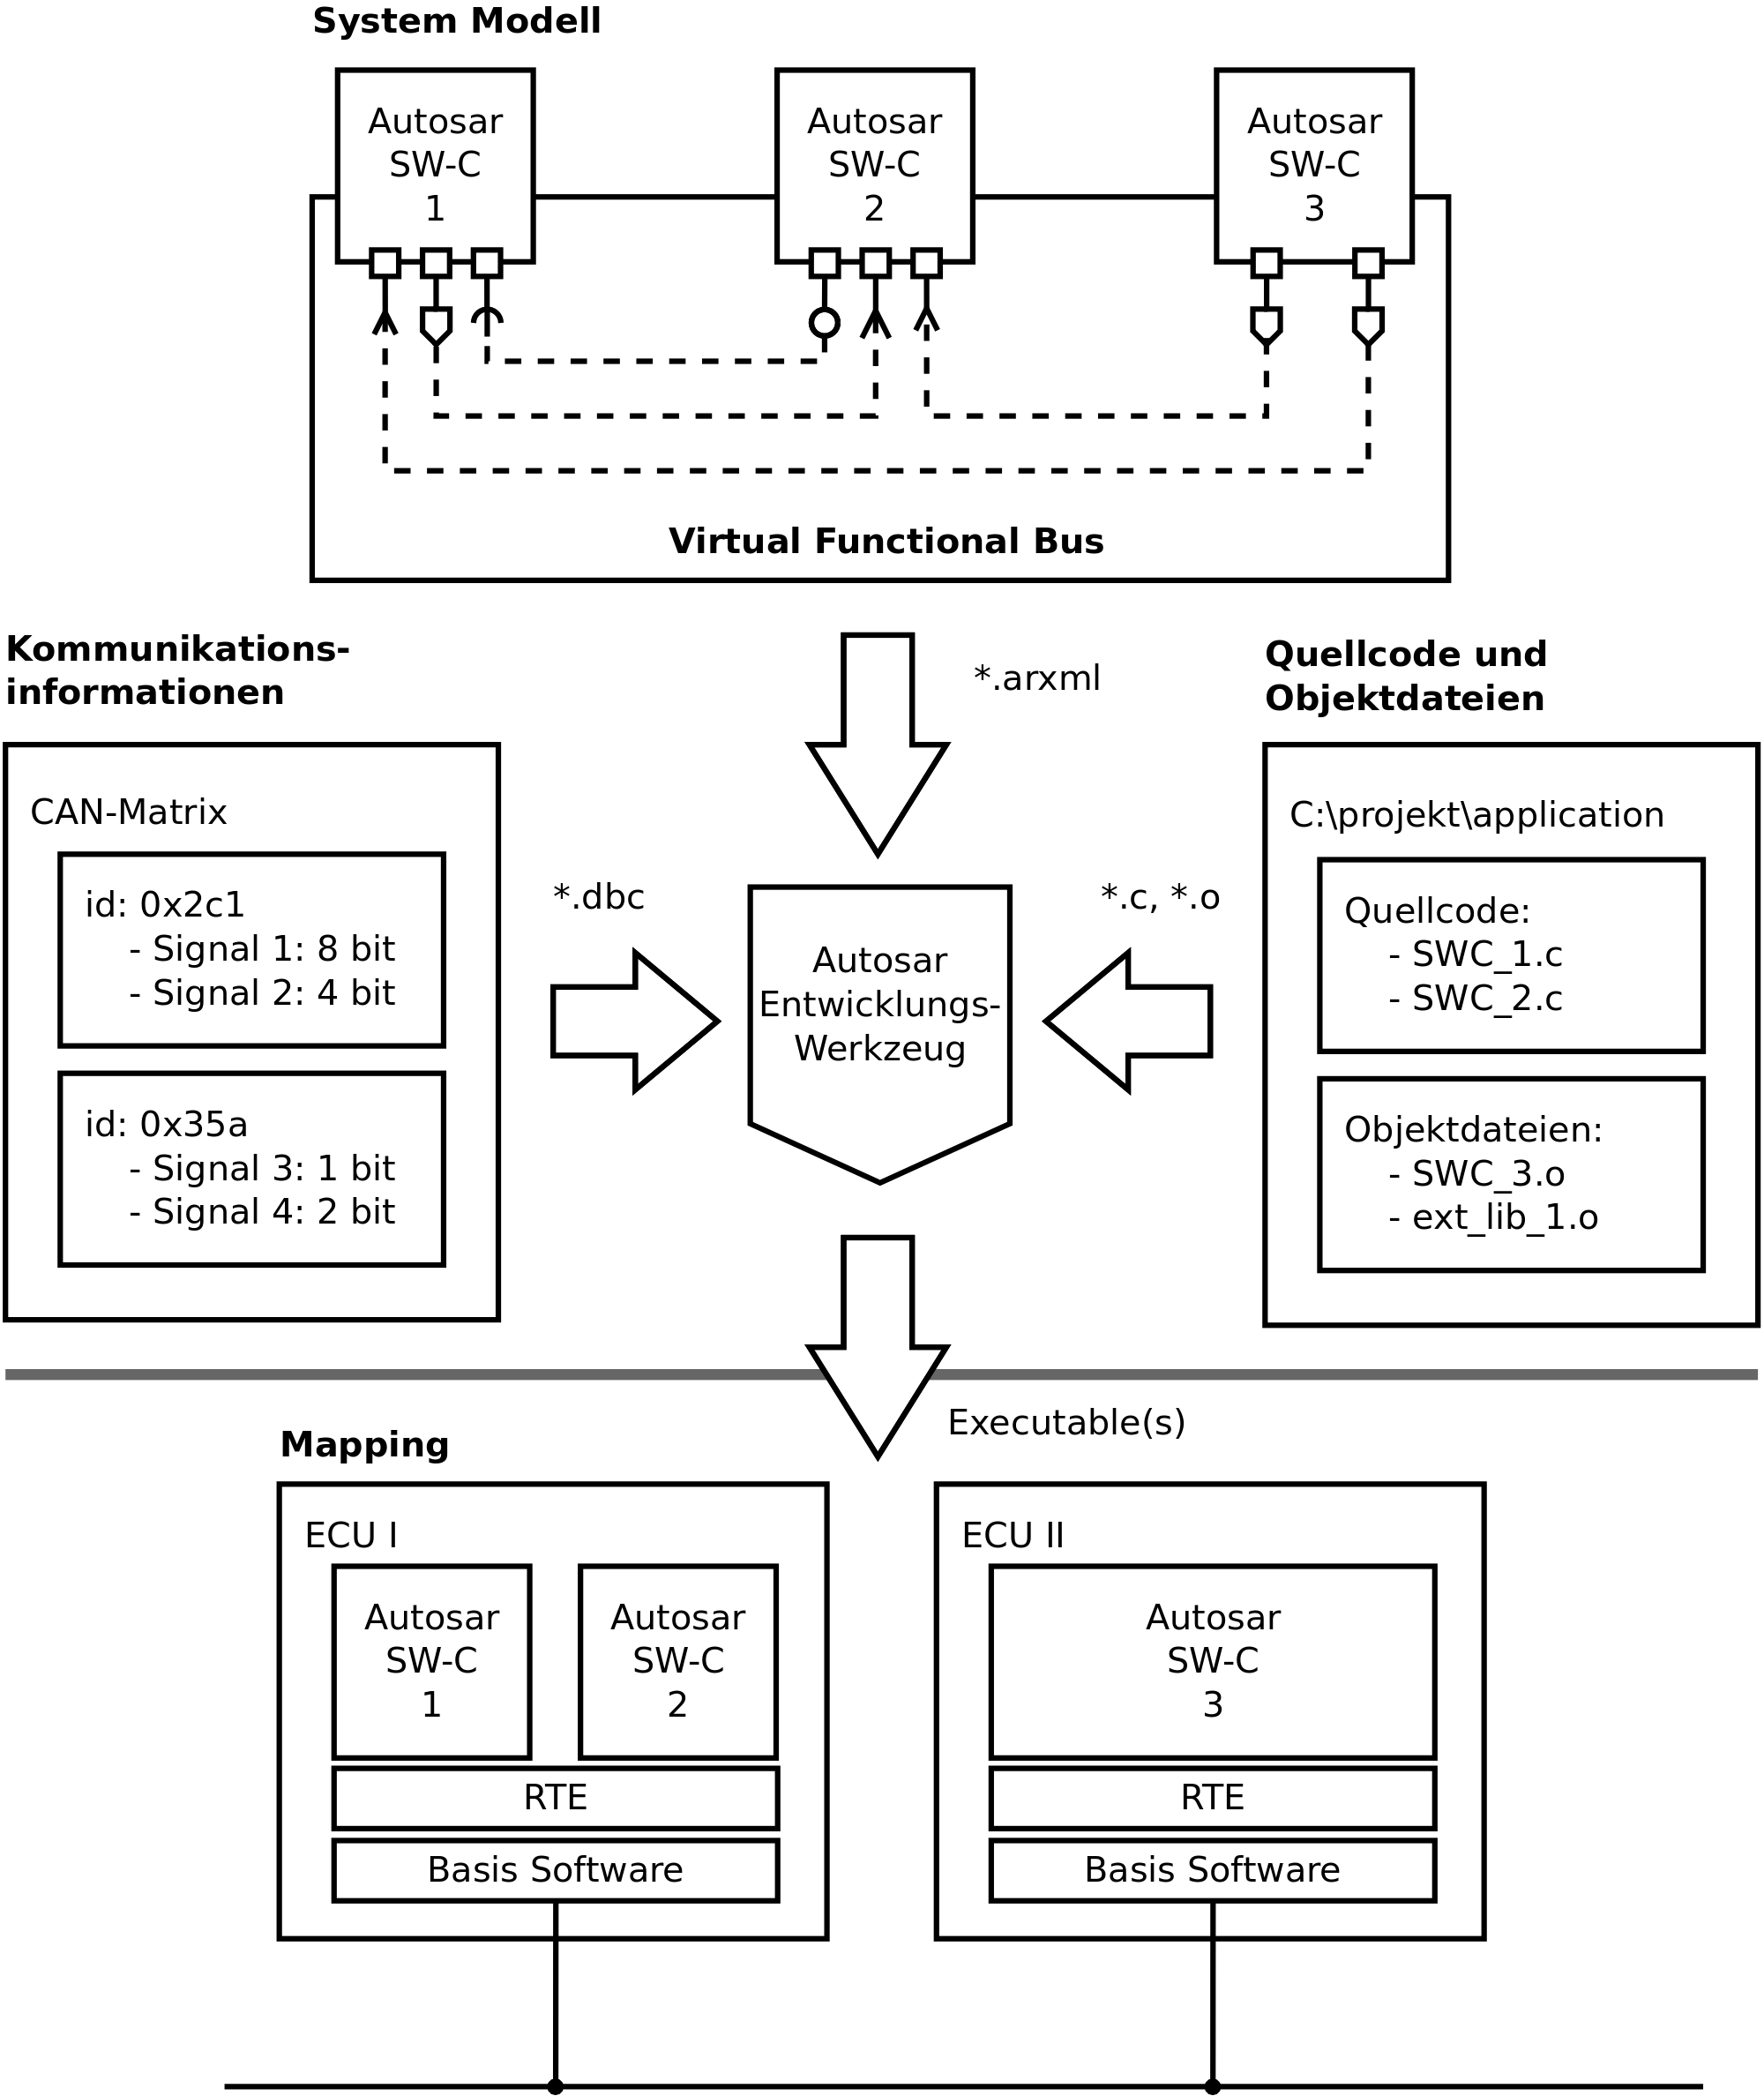
\includegraphics[width=1\textwidth]{autosar_overview.png}
\caption{Autosar Überblick}
\label{fig:autosar_overview}
\end{figure}

Der Lebenszyklus eines Autosar Systems lässt sich in zwei Phasen unterteilen. Die erste Phase ist in der Abbildung im oberen Teil zu sehen und beinhaltet das Design und die Entwicklung. In der zweite Phase werden alle Konfigurationen und Quelldateien verwendet um mittels des "`Autosar Entwicklungswerkzeugs"'  ausführbare Dateien zu generieren die anschließend auf der Ziel-Hardware ausgeführt werden können.

Zur Entwicklung eines Systems werden drei verschiedene Komponenten benötigt. Je nach Vorgabe können eine oder mehrere dieser Komponenten direkt von einem Hersteller oder OEM kommen, um so die Anforderungen für die restlichen Elemente zu beschreiben.

\paragraph{System Description} Ein Entwurf der "`System Description"' ist am oberen Rand der Abbildung zu sehen. Hier werden Komponenten und deren Verbindungen definiert. Die verschiedenen Interfaces und der Virtual Functional Bus werden in einem seperaten Abschnitt betrachtet. Komponenten (Software-Components, kurz SW-C) können beliebig geschachtelt werden um so eine logische Trennung zwischen Teil-Systemen zu schaffen. Hierbei ist lediglich zu beachten, dass pro ECU eine Top-Level-Composition (kurz TLC) gefordert wird. Die eigentliche Funtkionalität ist in Runnables implementiert. Diese müssen einer SW-C zugehören und werden von einem RTE-Event, zum Beispiel ein Timer, aktiviert.

Der Entwurf des Systems sollte genau überlegt sein, da dieser Grundstein für die weitere Entwicklung ist. In dieser Phase erfolgt auch die Zuriffskontrolle auf Interfaces sowie die Definition der RTE-Events, Zugriff auf Inter-Runnable-Variables und einer Reihe weitere Eigenschaften die später relevant sind.

Als Austauschformat wird XML, mit der Dateiendung "`.arxml"' verwendet. Es ist möglich nur einen Teil des Systems in eine XML-Datei zu exportieren um zum Beispiel einem OEM nur die für ihn relevante Teile offenzulegen.

\paragraph{Kommunikations-Informationen}
Um eine Kommunikation zwischen mehreren Komponenten zu ermöglichen müssen entsprechende Informationen geliefert werden. Hierbei existieren zum Beispiel die Formate DBC, FIBEX und LDF. Obwohl es sich bei DBC und LDF prinzipiell um Bus-Systemabhängige Formate handelt, spielt dies bei Autosar keine Rolle. So wird im Autosar-Stack die Kommunikations derart abstrahiert, sodass Botschaften transparent über unterschiedliche Bus-Systeme oder auch innerhalb einer ECU werden können.

Relevante Informationen sind Botschaften-IDs, Bezeichner, Bitlänge und Position der Signale in der Botschaft. Im Rahmen dieses Projektes werden DBC-Dateien mittels Vector CANoe erstellt.

\paragraph{Quellcode und Objektdateien}
Die eigentliche Implementation der Funktionalität findet im Quellcode, beziehungsweise im Objektcode statt. Durch den Autosar-Standard ist ein Benennungsschema definiert wodurch die entsprechenden Funktionen identifiziert werden. Auch der Zugriff auf Funktionen der RTE sind durch dieses Schema definiert. Die API-Funktionen der RTE werden vom RTE-Generator der verwendeten Autosar-Distribution erstellt. 

\paragraph{Autosar Entwicklungswerkzeug}
% Trennung zwischen den ...

\paragraph{VFB und RTE}

\paragraph{Basis Software}






% System-Entwurf
% - System-Description
% - UML
% - SW-C

% VFB und RTE
%   - Communication mechanisms

% BSW und Stack
%   - OS (OSEK as basis)
%   - MCAL
%   - Complex Driver



\subsection{Toolkette}
\label{sec:Toolkette}
% Verfügbare/Nötige Tools












%%%%%%%%%%%%%%%%%%%%%%%%%%%%%%% Netzwerk Managment %%%%%%%%%%%%%%%%%%%%%%%%%%%%%%%%%%
% Netzwerk Managment (!)
\section{Netzwerk Managment}
\label{sec:Netzwerk Managment}
% TODO




%%%%%%%%%%%%%%%%%%%%%%%%%%%%%%% Sicherheit ISO 26262 %%%%%%%%%%%%%%%%%%%%%%%%%%%%%%%%%%
\section{Sicherheit ISO 26262}
\label{sec:Sicherheit}
% TODO









%%%%%%%%%%%%%%%%%%%%%%%%%%%%%%% Umsetzung Fallbeispiel %%%%%%%%%%%%%%%%%%%%%%%%%%%%%%%%%%
% Gesamtes Modell darstellen
\chapter{Umsetzung des Fallbeispiels}
\label{sec:Umsetzung_Fallbeispiel}
% TODO





%%%%%%%%%%%%%%%%%%%%%%%%%%%%%%% Virtualisierung %%%%%%%%%%%%%%%%%%%%%%%%%%%%%%%%%%
\section{Virtualisierung}
\label{sec:Virtualisierung_Umgesetzt}
% TODO



% TODO: evtl Kapitel: Umsetzung Embedded Virt



%%%%%%%%%%%%%%%%%%%%%%%%%%%%%%% Kommunikation %%%%%%%%%%%%%%%%%%%%%%%%%%%%%%%%%%
\section{Kommunikation Linux und Autosar}
\label{sec:Kommunikation_L_A}
Eine Kommunikation zwischen Linux und Autosar kann auf verschiedene Wege erfolgen. Aus der klassischen Interprozess-Kommunikation sind Techniken wie Dateien, Messages, Semaphoren und Shared Mem bekannt. Diese stehen jedoch unter Autosar nicht zur Verfügung. Stattdessen können Client/Server und Sender/Receiver Interfaces verwendet werden die über verschiedene Schnittstellen nach außen geführt werden können. Im folgenden werden die drei Techniken CAN, Ethernet und VCAN betrachtet. Andere Bus-Systeme wie zum Beispiel LIN oder Flexray sind auch denkbar werden jedach im weiteren nicht näher untersucht. Der hier erwähnte VCAN bezeichnet den virtuellen CAN-Bus der bei Elektrobit tresos eingesetzt wird. Dieser tunnelt die CAN-Botschaften über eine Ethernet Verbindung und kann so CAN-Zugriff auf System ermöglichen die keine CAN-Schnittstelle besitzen. Vor- und Nachteile der Techniken sind im folgenden aufgeführt.

% TODO: hieraus eine Tabelle machen oder vielleicht als texte schreiben?!
\begin{itemize}
    \item CAN
    \begin{itemize}
        \item[$+$] Standard
        \item[$+$] Echtzeitfähig durch Arbitrierung
        \item[$-$] Linux benötigt vollen CAN Zugriff
        \item[$-$] Jedes Linux System CAN-Hardware (Kosten)
    \end{itemize}
    \item Ethernet
    \begin{itemize}
        \item[$+$] Standard
        \item[$+$] Hohe Übertragungsrate
        \item[$+$] Autosar soll "of the shelf"-TCP/IP-Stack verwenden der auch zu Linux kompatibel sein kann\cite[S. 21]{autosar_eth}
        \item[$-$] Kollisionen/Latenz und damit nur bedingt Echtzeitfähig
        \item[$-$] Benötigt Autosar 4.0
    \end{itemize}
    \item VCAN
    \begin{itemize}
        \item[$+$] Baut auf Ethernet auf
        \item[$+$] Gut umsetzbar im Evaluations-Prozess
        \item[$+$] Eigene "Logik" lässt sich im Gateway implementieren (Firewall, Kommunikations Matrix)
        \item[$-$] Nicht geeignet für Prouktiv-Systeme
        \item[$-$] Auf Elektrobit tresos beschränt
        \item[$-$] EB Gateway Protokoll muss implementiert werden
    \end{itemize}
\end{itemize}

% Warum VCAN?!
Sowohl die Kommunikation via Ethernet als auch CAN sind in diesem Projekt nicht weiter relevant, da beide nicht in der verwendeten Version 3.1 von WinCore zur Verfügung stehen. Somit wird in dieser Arbeit der VCAN betrachtet. Dieser ist einfach und flexibel und damit vor allem in den ersten Phasen eines Projektes von Vorteil.

% Deswegen VCAN-API geschrieben
Im Rahmen dieser Master-Arbeit wurde eine VCAN-API in Python entworfen die sowohl das Senden als auch Empfangen von CAN-Botschaften ermöglicht. Zusätzlich wurde die Funktionalität des von Elektrobit bereitgestellten Closed-Source VCAN-Gateways Reverse-Engineered werden. Lediglich die Anbindung an die PCAN-Hardware fehlt zur Zeit. Im folgenden Kapitel wird die API näher beschrieben.

% Der Quellcode steht unter der LGPL\footnote{Lizenz-Bedingung zu finden unter: \url{http://www.gnu.org/licenses/lgpl-3.0.txt}} und ist im Internet\footnote{VCAN-API Git Repository: \url{https://github.com/erebos42/VCAN_API}} zu finden.


\section{VCAN-API}
% Beschreibung der VCAN API







%%%%%%%%%%%%%%%%%%%%%%%%%%%%%%% Kommunikation %%%%%%%%%%%%%%%%%%%%%%%%%%%%%%%%%%
\section{Kommunikation Autosar und Scheinwerfer}
\label{sec:Kommunikation_A_S}
% TODO




%%%%%%%%%%%%%%%%%%%%%%%%%%%%%%% NM bei Autosar %%%%%%%%%%%%%%%%%%%%%%%%%%%%%%%%%%
% Netzwerk Managment (!)
\section{Zugriff auf Hardware (Netzwerkmanagment)}
\label{sec:AutosarNM}
% TODO








%%%%%%%%%%%%%%%%%%%%%%%%%%%%%%% Analyse des Fallbeispiels %%%%%%%%%%%%%%%%%%%%%%%%%%%%%%%%%%
\chapter{Analyse des Fallbeispiels}
\label{sec:Beispiel_Analyse}
% TODO




%%%%%%%%%%%%%%%%%%%%%%%%%%%%%%% Relevanz für die Wirtschaft %%%%%%%%%%%%%%%%%%%%%%%%%%%%%%%%%%
% Wie könnte das erarbeitete sinnvoll in der Wirtschaft umgesetzt werden?!
\section{Relevanz für die Wirtschaft}
\label{sec:Wirtschaft}
% TODO
% Es gibt bereits einige Embedded Hypervisor
% Multi-Core CPUs und leistungsfähige SOCs sind billig
% Sicherheit (ISO 26262) erfordert viel aufmerksamkeit
% Kurze "time-to-market" durch Evaluation auf Windows/Linux Platformen
% 



%%%%%%%%%%%%%%%%%%%%%%%%%%%%%%% Benchmark und Betrachtung der Echtzeitfähigkeit %%%%%%%%%%%%%%%%%%%%%%%%%%%%%%%%%%
% 
\section{Benchmark und Betrachtung der Echtzeitfähigkeit}
\label{sec:Benchmark}
% TODO




%%%%%%%%%%%%%%%%%%%%%%%%%%%%%%% Sicherheit bei Embedded Virtualisierung %%%%%%%%%%%%%%%%%%%%%%%%%%%%%%%%%%
\section{Sicherheitsbetrachtung des Fallbeispiels}
\label{sec:Sicherheit_Beispiel}
% TODO












%%%%%%%%%%%%%%%%%%%%%%%%%%%%%%% Zusammenfassung %%%%%%%%%%%%%%%%%%%%%%%%%%%%%%%%%%
\chapter{Fazit und Ausblick}
\label{sec:FazitAusblick}
% TODO










%%%%%%%%%%%%%%%%%%%%%%%%%%%%%%%%%%% Anhang %%%%%%%%%%%%%%%%%%%%%%%%%%%%%%%%%
\backmatter
\appendix
\part*{Anhang}


%%%%%%%%%%%%%%%%%%%%%%% Erklärung und CD %%%%%%%%%%%%%%%%%%%%%%%%%%%%%
\chapter{Erklärung}
\label{sec:Erklärung}
Hiermit erkläre ich, dass ich die vorliegende Arbeit selbstständig und nur unter Verwendung der angegebenen Quellen und Hilfsmittel erstellt habe.
\vspace{2.5cm} \par
Wolfenbüttel, den % TODO


\chapter{Beigelegte CD}
\label{sec:BeigelegteCD}



%%%%%%%%%%%%%%%%%%%%%%%%%%%%%%% Bibliographie %%%%%%%%%%%%%%%%%%%%%%%%%%%%%%
% \setbibpreamble{Die Quellenangaben sind alphabetisch nach den Namen der Autoren sortiert.
% Bei mehreren Autoren wird nach dem ersten Autor sortiert.\par\bigskip\bigskip}
%
% Quellen, die nicht direkt zitiert wurden, aber trotzdem hier erscheinen sollen!
%\nocite{tbinformatik}\nocite{tb_et2000}\nocite{tb_mathe1999}
\nocite{*}
%
\begin{singlespace}
\bibliographystyle{natdin}	% alphadin, plaindin, abbrvdin, unsrtdin, natdin
					            % germbib: gerabbrv, geralpha, gerplain, gerunsrt, gerapali, gerxampl
                           		% plainnat, abbrvnat, unsrtnat
                           		% Am besten geeignet: natdin
                           		% oder was ist mit dinat
                           		% ???apalike???
\bibliography{literature}
\end{singlespace}
%%%%%%%%%%%%%%%%%%%%%%%%%%%%%%%%%%%%%%%%%%%%%%%%%%%%%%%%%%%%%%%%%%%%%%%%%%%%

\end{document}


